
\documentclass{article}
\usepackage[utf8]{inputenc}

\title{TT3010 - Audio technology and room acoustics. \newline Exercise 1}
%\author{Jan Arne Bosnes}
\date{\today}

\usepackage{natbib}
\usepackage{graphicx}
\usepackage{multicol}
\usepackage{gensymb}
\usepackage{float}

\newcommand\myfigure[1]{%
\medskip\noindent\begin{minipage}{\columnwidth}
\centering%
#1%
%figure,caption, and label go here
\end{minipage}\medskip}


\begin{document}

\maketitle

All tasks are reproduced from chapter 23 in "Science of Sound". %It is recommended that the student will try to do every task (except when a task is marked \textit{This task is for a later chapter}), but t
Tasks marked \textit{Mandatory} must be handed in for approval (online). Deadline is specified in blackboard. 
%Some tasks, as marked, are for a later chapter.

\section*{Tasks}
%\begin{multicols}{2}
\begin{itemize}
    \item [1.] \textit{Mandatory}. Using the Table 23.1, compare the absorption of 100m$^2$ of plastered wall with that of 100m$^2$ of a carpeted floor at 
        \begin{itemize}
        \item [a.] 125Hz;
        \item[b.] 2000Hz.
        \end{itemize}
    
    \item[2.] \textit{Mandatory}. An auditorium has dimensions 40m*20m and a ceiling height of 15m. The front and back walls are covered with plywood paneling; the side walls and ceiling are plaster. The floor is wood. There are 1100 upholstered seats. Estimate the reverberation time (at 500Hz) when
            \begin{itemize}
        \item [a.] The hall is empty;
        \item[b.] Half the seats are filled;
        \item[c.] All the the seats are occupied.
        \end{itemize}
        
    \item[3.] \textit{Mandatory}. Estimate the time decay t1 of the first reflected sound for a person seated near the center of the auditorium described in Question 2. Does the first reflection arrive from the side or from overhead ?
    
    \item[4.]  If the ceiling in the auditorium were covered with acoustical tile, by how much would the reverberation time be decreased ?
    
    \item[5.] \textit{Mandatory}. Specify reasonable values for the reverberation times at 100, 200 and 1000Hz for a 2000m$^3$ concert hall to be used primarily for orchestral music.
    
    \item[6.] \textit{Mandatory}. If two hard parallel walls are spaced 30m apart, calculate the repetition rate of the flutter echo that might result. What efforts might be made to prevent its occurence ?
    
    \item[7.] Find the reverberation time at 8000Hz for a very live room having a volume of 1000m$^3$ when the temperature is 20\degree C and the relative humidity is 30\%. Assume that absorption by the walls is negligibly small. Would your answer be different if V = 100m$^3$ instead ?
    
 
\end{itemize}

%\end{multicols}

\begin{figure}[H]
    \centering
    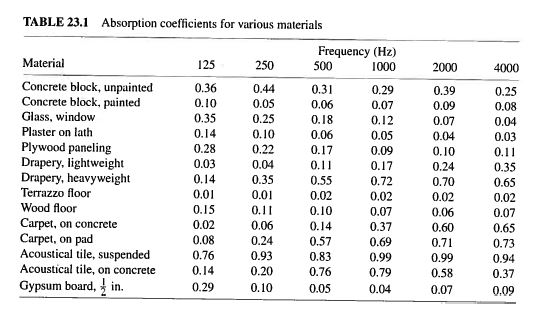
\includegraphics[scale=0.9]{figures/table23_1.jpg}
   \caption{Retrieved from Rossing chap 23.}
    \label{fig:nc}
\end{figure}

\begin{figure}[H]
    \centering
    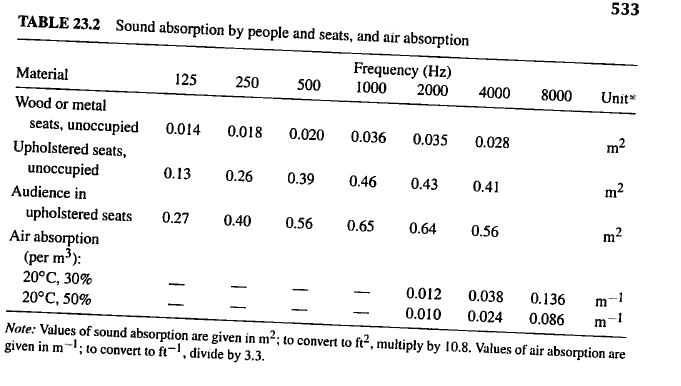
\includegraphics[scale=0.8]{figures/table23_2.jpg}
   \caption{Retrieved from Rossing chap 23.}
    \label{fig:nc}
\end{figure}

\begin{figure}[H]
    \centering
    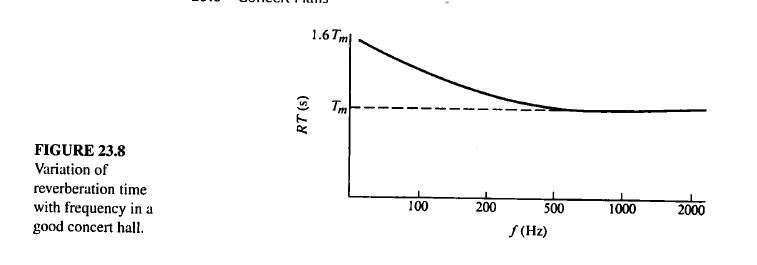
\includegraphics[scale=0.8]{figures/figure23_8.jpg}
   \caption{Retrieved from Rossing chap 23.}
    \label{fig:nc}
\end{figure}


\begin{figure}[H]
    \centering
    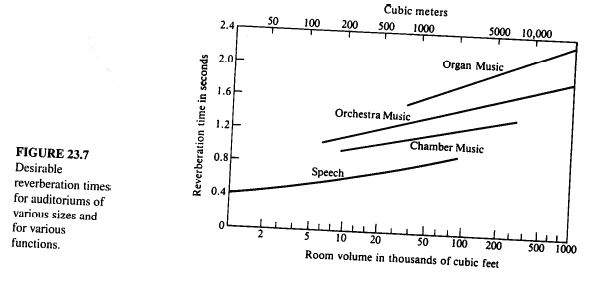
\includegraphics[scale=0.9]{figures/figure23_7.jpg}
   \caption{Retrieved from Rossing chap 23.}
    \label{fig:nc}
\end{figure}
\end{document}
